\cotefile{37}
\scanpage{52}
\noindent SGA 5 \(\overline{\underline{\mathrm{VII}}}\)\quad th de Lefschetz faible sans \unsure{supposer} \(X\) ni \(Y\) lisses (seulement \(X-Y\) lisse \ldots)

\noindent SGA 5 \(\overline{\underline{\unsure{\mathrm{V}|\mathrm{VI}}}}\)\quad \(\mathbb{Q}_{\ell}\)-faisceau : signaler définition raisonnable en termes de \uline{champ} \uline{associé}

% The replacement VI is below the cancelled numeral, within an open U-shaped curve.
\noindent SGA 5. \tikz[baseline=(old.base),x=1cm,y=1cm]{
\node[inner sep=0pt] (old) at (0,.44) {\(\deleted{\overline{\underline{\unsure{\mathrm{IV}|\mathrm{V}|\mathrm{VI}}}}}\)};
\node[inner sep=0pt] (vi) at (0,-.16) {\inserted{\(\overline{\underline{\mathrm{VI}}}\)}};
\draw[thin] (-.39,.06) .. controls (-.45,-.70) and (.42,-.73) .. (.76,.49);
}\quad Reprendre en langage de \(\mathbb{Z}_{\ell}\)-faisceaux ou\textsuperscript{\inserted{\unsure{*|+}}} \(\mathbb{Q}_{\ell}\)-faisceaux les notions essentielles dont il a été question dans SGA 4 (, Ajouter nouveau N\textsuperscript{\uline{o}}).

\noindent SGA 5 \(\overline{\underline{\mathrm{IV}}}\)\quad Essayer de faire dans le cas relativement lisse ttes les constructions essentielles

\figure{
\begin{tikzpicture}[x=\linewidth,y=1cm]
\draw[thin] (0,0) .. controls (.23,.12) and (.49,.08) .. (.62,.06)
 .. controls (.77,.05) and (.90,-.03) .. (.96,.02);
\end{tikzpicture}}

\noindent \(\overline{\underline{\mathrm{VI}}}\)\quad \unsure{Systèmes|Système} projectifs \inserted{\tikz[baseline=(adiques.base)]{
\node[inner sep=0pt] (adiques) {adiques};
\draw[thin] ([xshift=-.35em,yshift=-1.2ex]adiques.south west)
 .. controls +(90:1.6ex) and +(-1em,-.2ex) .. (adiques.south)
 .. controls +(1.8em,.2ex) and +(0em,-1.1ex) .. ([xshift=1.1em,yshift=.3ex]adiques.east);
}} dans les catégories \unsure{dérivées} \ldots\ (ou dans thèse)

% Two faint isolated traces below the parenthesis; no lexical identity is assigned.
\figure{\begin{tikzpicture}[x=\linewidth,y=1cm]
\path[use as bounding box] (0,-.45) rectangle (1,.35);
\node[anchor=west,inner sep=0pt] at (.35,.08) {\unsure{\tikz[baseline=-.5ex,x=1cm,y=1cm]{\draw[thin,gray] (0,0) -- (.09,.04) -- (.17,-.01) -- (.19,.10) -- (.23,.16) -- (.27,.21); \draw[thin,gray] (.23,.16) -- (.21,.20);}}};
\node[anchor=west,inner sep=0pt] at (.45,-.18) {\unsure{\tikz[baseline=-.5ex,x=1cm,y=1cm]{\draw[thin,gray] (.08,.24) .. controls (.07,.19) and (.08,.15) .. (.08,.11) -- (.02,.15) -- (0,.08); \draw[thin,gray] (.08,.11) -- (.15,.02); \draw[thin,gray] (.03,-.04) -- (.08,-.10) -- (.14,-.04); \fill[gray] (.08,-.14) circle (.015);}}};
\end{tikzpicture}}
% slanted: a detached pair of dots, possibly incidental rather than a colon
\margin{\unsure{\tikz[baseline=-.3ex]{\fill (0,0) circle[radius=.35pt];\fill (.07,.10) circle[radius=.35pt];}}}

\noindent SGA 5 \(\mathrm{V}\)\quad dans introduction du \unsure{livre|Hom} ou de l'expo\unsure{sé} signaler l'ennui des coeff. trop particuliers \((\mathbb{Z}_{\ell},\,\unsure{\mathbb{Z}|Z}/\ell^{\unsure{\nu|n|N}}\mathbb{Z}\ -\,-)\)

\figure{
\begin{tikzpicture}[x=\linewidth,y=1cm]
\draw[thin] (0,.03) .. controls (.12,.11) and (.19,.04) .. (.29,-.02)
 .. controls (.39,-.08) and (.45,.02) .. (.57,.01)
 .. controls (.74,.02) and (.85,-.11) .. (.91,-.06);
\end{tikzpicture}}

\noindent \(\mathrm{I}\)\quad \S\ 5\qquad Donner, si \(i\unsure{{<}|{:}|{\in}}\unsure{\eta|y}\overset{\unsure{\sim}}{\longrightarrow} X\) inclusion du p\textsuperscript{t} générique, et \(F_{\eta}\) Module loc. \unsure{libre} sur \(\eta\)
\[
 D\bigl(i_{*}(F_{\eta})\bigr)=i_{*}\bigl(D(F_{\eta})\bigr)
\]
% archive sheet number: 51
\clearpage
\scanpage{53}
% letterhead
\begin{center}
{\sffamily INSTITUT\\
DES HAUTES ÉTUDES SCIENTIFIQUES}\\[-0.4ex]
\rule{1.7cm}{0.5pt}
\end{center}

\noindent SGA \textbf{5}\qquad \(\overline{\underline{\mathrm{XIII}}}\)

\figure{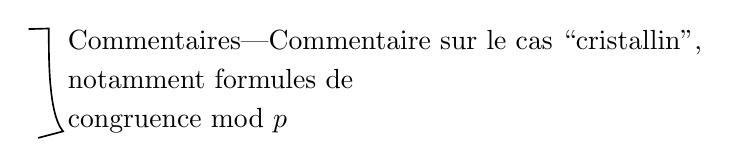
\begin{tikzpicture}
\node[anchor=west,inner sep=0pt,align=left] (lignes) {\unsure{Commentaires|Commentaire} sur le cas ``cristallin'',\\[0.5ex]
notamment formules de\\[0.5ex]
congruence \(\mathrm{mod}\ p\)};
\draw[semithick] ([xshift=-1.4em,yshift=0.05ex]lignes.north west) --
 ([xshift=-0.67em,yshift=0.10ex]lignes.north west)
 .. controls ([xshift=-0.65em,yshift=-1ex]lignes.north west)
 and ([xshift=-0.75em,yshift=1.8ex]lignes.south west)
 .. ([xshift=-0.15em,yshift=0.20ex]lignes.south west) --
 ([xshift=-1.05em,yshift=-0.35ex]lignes.south west);
\end{tikzpicture}}

\noindent \deleted{\illegible{1}}\quad \(\overline{\underline{\mathrm{IV}}}\)\qquad Faire attention au cas relatif, consulter \(\overline{\underline{\mathrm{VII}}}\) et SGA 6 \(\overline{\underline{\mathrm{X}}}\)

\noindent \(\overline{\underline{\mathrm{XIV}}}\)\quad (\unsure{Problèmes|Problémes} et \unsure{Commentaires|Commentaire})

Signaler les variantes \(\mathrm{mod}\ p\) et \unsure{Variantes|variantes} cristallines (cf \unsure{une|mes} \unsure{note|notes} à propos th. de Katz).
% archive sheet number: 52
\clearpage
\scanpage{54}
% upper right, boxed pencil note
\margin{\figure{
\begin{tikzpicture}[baseline=(copie.base)]
\node[align=left,inner sep=4pt] (copie) {Faire copie\\pour Jouanolou};
\draw[thin] ([xshift=-3pt,yshift=1pt]copie.north west) .. controls ([xshift=4pt,yshift=1pt]copie.north west) and ([xshift=-5pt,yshift=4pt]copie.north east) .. (copie.north east) -- ([yshift=-4pt]copie.north east);
\draw[thin] ([yshift=-1pt]copie.north west) -- (copie.south west) -- ([xshift=2pt,yshift=1pt]copie.south east) -- ([xshift=4pt,yshift=-12pt]copie.north east);
\end{tikzpicture}}}
% letterhead
\begin{center}
{\sffamily HARVARD UNIVERSITY\\
CAMBRIDGE, MASSACHUSETTS 02138}
\end{center}
% letterhead
\noindent {\sffamily DEPARTMENT OF MATHEMATICS\\
2 DIVINITY AVENUE}\\
\hfill Aug 4, 1969\\
% isolated mark at the far right of the date; function unassigned
\margin{\figure{\begin{tikzpicture}[x=1mm,y=1mm]\fill (0,0) .. controls (-0.35,0.05) and (-0.38,0.36) .. (-0.16,0.40) .. controls (0.01,0.45) and (0.11,0.18) .. (0.29,0.31) .. controls (0.40,0.17) and (0.31,-0.12) .. (0.12,-0.06) -- cycle;\end{tikzpicture}}}

\noindent Dear Grothendieck,\\

I have been reading recently some notes from the IHES (one of your seminars, I suppose) entitled ``Exposé \(\overline{\underline{\mathrm{V}}}\). Systèmes
\reversemarginpar\margin{\figure{
\begin{tikzpicture}[x=1cm,y=1cm]
\draw[thin] (0,1.10) -- (-0.01,0.13) .. controls (-0.01,0.06) and (0,0.02) .. (0.02,0);
\end{tikzpicture}}}\normalmarginpar%
projectifs J-adiques, par J.P. Jouanolou.'' Could you tell me (for purposes of reference) to which seminar they belong, and whether there is a more recent edition?

Also I have some comments and questions. The most serious question is that I do not understand the proof of the ``Theorem of Shih'', \unsure{A.3.1|A.3.1.} on page 46. It seems to me that the lemma on p. 45 is valid only for \(r>p\) (cf EGA \(\unsure{0|O}_{\overline{\underline{\mathrm{III}}}}\) 13.5.5.2), and so \deleted{\unsure{the|from}} the equivalence of statements (i) and (ii) of the theorem is not clear. (I do agree, however, with the weaker statement ``(resp.\ldots)'' in parentheses). This casts doubt on the following theorem A.3.2 on p. 47, and also on the earlier Prop. 5.3.1 on p. 40. These difficulties would disappear if one worked \unsure{throughout|throughtout} in the category \(\mathrm{pro}\text{-}A\) \margin{\figure{\unsure{\begin{tikzpicture}[x=1mm,y=1mm]
\fill (0,0) .. controls (-0.28,0.02) and (-0.25,0.24) .. (-0.08,0.35) .. controls (0.08,0.43) and (0.26,0.10) .. (0.20,0.03) -- cycle;
\fill (0.55,0.92) .. controls (0.30,0.83) and (0.35,1.13) .. (0.48,1.27) .. controls (0.59,1.48) and (0.81,1.20) .. (0.76,1.06) -- cycle;
\end{tikzpicture}}}} of projective systems with the usual equivalence, rather than in the \deleted{category} finer category \(P_{AR}\).

Other comments: p. 42 line \(\dot{-}1\). Isn't the spectral sequence actually biregular in case of a finite filtration?

p. 47 line \(-1\). I think the hypothesis should be stated for \(n\) and \(n+1\), instead of \(n\) and \(n-1\) (cf EGA \(0_{\overline{\underline{\mathrm{III}}}}\) 11.1.10).
% archive sheet number: 53
\clearpage
\scanpage{55}
\mspage{2}

\noindent p. 38\quad I believe the artinian hypothesis in this proposition is unnecessary, if one assumes that \(X\) and \(Z\) are both \inserted{AR}-\(J\)-adic noetherian. To be precise, let

% The two text rows occupy the same cells spanned by the three upward arrows.
\diagram{\begin{tikzcd}[ampersand replacement=\&,column sep=1em,row sep=0.6ex]
0 \arrow[r] \& X \arrow[r] \& Y \arrow[r] \& Z \arrow[r] \& 0\\
\&\& \makebox[0pt][c]{\parbox{0.96\linewidth}{\raggedright
be an exact sequence of projective systems of \(A\)-modules, such that
\(J^{n+1}X_n=J^{\unsure{n+1|n+{}}}Y_n=J^{n+1}Z_n=0\) for all \(n\), and assume \(X\) and \(Z\) are AR-\(J\)-adic noetherian. Then \(Y\) is also AR-\(J\)-adic noetherian.\par
\smallskip\noindent Indeed, taking \(\underset{\longleftarrow}{\lim}\) we get an exact sequence}} \&\&\\
0 \arrow[r] \& M' \arrow[r] \& M \arrow[r] \& M'' \arrow[r] \& 0\\
\&\& \makebox[0pt][c]{\parbox{0.96\linewidth}{\raggedright
of \(A\)-modules, with \(M',M''\) finite type, so \(M\) is also finite type.
let \(\mathbb{A}\) be the projective system \((A/J^{n+1})_n\). Then by Artin-Rees, we have an exact sequence}} \&\&\\
0 \arrow[r] \& M'\otimes\mathbb{A} \arrow[r] \arrow[uuuu,thin,start anchor=north east,end anchor=south west,bend left=4] \&
M\otimes\mathbb{A} \arrow[r] \arrow[uuuu,thin,start anchor=north east,end anchor=south,bend left=3] \&
M''\otimes\mathbb{A} \arrow[r] \arrow[uuuu,thin,start anchor=north east,end anchor=south east,bend left=2] \& 0
\end{tikzcd}}

\noindent in the category \(P_{AR}\) of projective systems up to translation. There is a natural map of this sequence to the first. The two outside arrows are isomorphisms, so \(M\otimes\mathbb{A}\xrightarrow{\approx}Y\), which \unsure{shews|shows} that \(Y\) is AR-\(J\)-adic.

I came to these questions while \deleted{\illegible{1}} working on my paper ``Affine Duality and Cofiniteness'' which I am finally preparing for publication. \margin{\figure{\unsure{\begin{tikzpicture}[x=1mm,y=1mm]
\fill (0,0) .. controls (-0.24,0.01) and (-0.26,0.20) .. (-0.06,0.33) .. controls (0.09,0.40) and (0.25,0.12) .. (0.19,0.03) -- cycle;
\fill (0.55,0.97) ellipse[x radius=0.18,y radius=0.24,rotate=-25];
\end{tikzpicture}}}}I will send you a copy when it is ready.

\noindent\hfill Sincerely yours,\\
\null\hfill R. Hartshorne\\
% archive sheet number: 54
\clearpage
\scanpage{69}
\mspage{\handwritten{- 4 -}}

p.37, li.6 : ``composé'' au lieu de ``composée''.

\begin{center}
Commentaires Appendice
\end{center}

p.3 : détailler preuve de 7.4 ? ($Y$ plat sur $S$, ... il en résulte aisément ..., on vérifie aisément ...)

p.1 : dans l'énoncé 7.1, de quel $K^{\bullet}$ s'agit-il ?

p.5, li.5 : réf. pour \handwritten{``}$X_t$ et $X_s$ réguliers $\handwritten{\Rightarrow}$\handwritten{\unsure{``|''}}$X$ régulier\handwritten{''}.

p.6, li.6 : peut-on voir l'argument ?

p.7, li.8 du bas : ``Ce résultat généralise 7.5'' (une fois qu'on a remarqué que, pour $X = S$, les flèches du diagramme de 7.3 sont les flèches identiques de $\underline{Z}$.)

p.7, li.5 du bas : ``récrire'' et non ``réécrire''.

p.8, li.12 du bas : ``horizontales'' et non ``verticales''.

p.8, li.6 du bas : ``du prisme'' et non ``du carré''.

p.9 : nommer les flèches verticales d\deleted{a}e (7.10.2 bis).

p.9, li.6 : ajouter ``(cf. 3.3)'' après \unsure{```|``}implique''.

% Detached marks retain uncertain authorship; small inline boxes preserve their relative placement.
p.9 : références pour $\mathrm{Gr}^{\bullet}_{\mathrm{top}}$ et l'assertion de compatibilité aux filtrations ?\hspace{0.4em}\raisebox{0.35ex}[0pt][0pt]{\parbox[c]{2mm}{\figure{\unsure{\begin{tikzpicture}[x=1mm,y=1mm,baseline=0pt]
\fill (0,0) .. controls (-0.12,0.12) and (-0.09,0.42) .. (0.02,0.52)
 .. controls (0.15,0.63) and (0.30,0.43) .. (0.28,0.24)
 .. controls (0.28,0.06) and (0.14,-0.03) .. (0,0) -- cycle;
\end{tikzpicture}}}}}

Donner aussi le diagramme analogue à (7.10.1 bis) avec \makebox[0pt][l]{\hspace{0.70em}\raisebox{-1.45ex}[0pt][0pt]{\parbox[c]{2mm}{\figure{\unsure{\begin{tikzpicture}[x=1mm,y=1mm,baseline=0pt]
\fill (0,0) .. controls (-0.12,0.10) and (-0.17,0.35) .. (0.01,0.42)
 .. controls (0.16,0.48) and (0.36,0.30) .. (0.25,0.14)
 .. controls (0.17,0.03) and (0.07,-0.05) .. (0,0) -- cycle;
\fill (0.60,1.13) ellipse[x radius=0.34,y radius=0.17,rotate=45];
\end{tikzpicture}}}}}}$\mathrm{Gr}^{\bullet}(\ )_{\underline{Q}}$ pour $g$ projectif, d'intersection complète, et de dimension relative virtuelle donnée.

p.10, li.11 : ``standard'' et non``standart''.

p.10, li.13 : ne faut-il pas ajouter ``connexe'' après ``schéma algébrique'' et ``courbe algébrique'' ? Y a-t-il une référence à l'intention du lecteur qui aimerait voir une démonstration d\deleted{d}e l'assertion en question?

% archive sheet number: 68
\clearpage
\scanpage{70}
\mspage{\handwritten{- 5 -}}

p.11, li.7 du bas : $K^{\bullet}(T)$ et non $K_{\bullet}(T)$.

p.11, li.18 : il devrait y avoir une référence dans Exp.V pour cette assertion.

p.11, li.11 du bas : référer à (3.1) pour la structure de module envisagée.

p.11, li.9 du bas : ``ci-dessus'' et non ``ci-dessous''. Apparemment les définitions garderaient un sens en supposant seulement $C$ connexe, ou est-ce que je me canule ?

p.12,li.6 : ``on se ramène immédiatement ...'' : bref, on utilise la compatibilité de la spécialisation au changement de trait\handwritten{(7\unsure{-|.}15)}\unsure{\handwritten{.}|.}

p.12, li.6 du bas : ``donc il existe (cf. EGA IV 2.8) ...''

p.12, li.3 du bas : ``on peut choisir pour $C$ un schéma régulier'', mais plus nécessairement plat sur $S$.

p.13, li.2 : ``il est bien connu (SGA ou EGA ? ) ...''

\handwritten{p.13, li.10 du bas : ($\overline{\underline{\mathrm{IV}}}$ 2.12) au lieu de ($\overline{\underline{\mathrm{III}}}$ 2.12).}

p.13, li.3 du bas : il semble qu'on utilise le fait déjà cité(sans référence) que par $x_{\unsure{o|0}s}$ et $x_{\unsure{l|1}s}$ passe une courbe connexe.

p.14, li.10 : ``propre et lisse'' ne suffit-il pas ?

p.15, li.10 : ``donne naissance à '' plutôt que ``provient de''.

p.16, li.14 : au lieu de ``par Krull-Akizuki'' dire plutôt ``comme $S$ est hensélien''.

p.16, li.16 : $X$ n'étant pas supposé plat, le fait que les fibres soient géométriquement régulières n'implique pas, il me semble, que $X$ soit lisse.

\handwritten{p.16, li.8 du bas : ``on trouve\makebox[0pt][l]{\hspace{0.15em}''}\unsure{\ldots|.\,:|.\,.|.} ajouter ``(cf. 7.16)''.}

p.17, 7.13.6 : les points importants, à savoir :
\begingroup
\makeatletter\tagsleft@true\makeatother
\[
\handwritten{\psi}_i(c^i(x)) = (-1)^{i-1}(i-1)!\;c^i_{\unsure{\chi|\handwritten{\chi}}}(x)\quad,\tag*{(i)}
\]
\[
\handwritten{\psi}_{i+j}(c^i(x)c^j(y)) = (-1)^{i+j-1}(i+j-1)!c^i_{\chi}(x)c^j_{\chi}(y)\quad,\tag*{(ii)}
\]
\endgroup
pour lesquels on peut référer à (V \handwritten{6}.\handwritten{5}.\handwritten{3} et \handwritten{6}.\handwritten{6}.\handwritten{4}), ne sont pas
% archive sheet number: 69
\clearpage
\scanpage{71}
\mspage{\handwritten{- 6 -}}
\deleted{mis} mis en lumière (c'est mieux expliqué dans XIV 5.1 et 5.2) ; la référence (V 3.3.2) est vide.

p.18, li.3 : supprimer ``commutatifs''.

p.18, li.5 du bas : ``qu'on laisse au lecteur le soin d'écrire''.

p.19, li.3 : est-ce vraiment possible sans autre hypothèse sur $Z$ ?

p.19, li.7 : ``linéairement'' = ``rationnellement'' ?

p.19, li.15 : ``standard'' et non ``standart''.

p.19, li.11 du bas : ``une conjecture équivalente ...'' : on utilise implicitement le fait que $\mathrm{Gr}^{\bullet}\handwritten{\xrightarrow{\sim}}\mathrm{Gr}^{\bullet}_{\mathrm{top}}$ modulo torsion (VII\hspace{2em}).

p.19, li.3 du bas : référer à (SGA 5 IV\hspace{2em}).

p.20, li.10 : référer à (EGA IV 2.8) pour $Z$ plat sur $S$. Il faudrait aussi une référence pour le fait que $\dim(Z_s) = \dim(Z_t)$.

p.20, li.16 : ``rationnelle'' et non ``rationelle''. De même, 2 lignes plus bas, ``rationnellement'' et non ``...''. N'est-il pas prudent de supposer $f$ lisse ?

% Two faint detached traces above the final e; authorship and function unresolved.
p.20, li. 3 du bas : manque flèch\makebox[0pt][l]{\hspace{0.05em}\raisebox{2.0ex}{\parbox{0.8em}{\figure{\unsure{\begin{tikzpicture}[x=1mm,y=1mm,baseline=0pt]
\fill[gray!65] (0,0) ellipse[x radius=0.28,y radius=0.12,rotate=12];
\fill[gray!65] (0.62,1.03) ellipse[x radius=0.12,y radius=0.34,rotate=-9];
\end{tikzpicture}}}}}}e.

p.22, li.8 : ``On peut donc prendre (cf. IV 2.12) ...''.

p.2\deleted{\unsure{Z|2|3}}2, li.5 : Supposer $X$ plat sur $S$.

p.23, li.2 : hypothèses sur $X$ ?

p.23, dernière ligne : donner le corollaire pour $\mathrm{NS}$ ?

% Short left-margin stroke, level with the upper part of the following reference.
\noindent\makebox[0pt][r]{\raisebox{0.75ex}[0pt][0pt]{\parbox[b]{8.8mm}{\handwritten{\figure{\begin{tikzpicture}[x=1mm,y=1mm]
\draw[line width=0.35pt,line cap=round] (0,0) .. controls (2.1,0.20) and (5.7,0.22) .. (7.0,0.10) .. controls (7.5,0.04) and (7.9,0.04) .. (8.2,0.03);
\end{tikzpicture}}}}}}p.24, li.3 : supprimer ``localement''(canular à la li. 11).

p.24, li.6 : ``on note (EGA II 7.1.9) ...''.

% The detached pair after et is reproduced by shape; its function and origin remain uncertain.
p.24, li.11 : références pour ``essentiellement de type fini'' et\hspace{0.6em}\raisebox{0.45ex}{\parbox[b]{2.0mm}{\figure{\unsure{\begin{tikzpicture}[x=1mm,y=1mm]
\fill (0,0) ellipse[x radius=0.26,y radius=0.21];
\fill (0.70,1.02) ellipse[x radius=0.22,y radius=0.34,rotate=-23];
\end{tikzpicture}}}}} ``universellement japonais'' ?

% The long left-margin stroke reaches across the upper part of p.24.
\noindent\makebox[0pt][l]{\hspace{-37.5mm}\raisebox{-1.4ex}[0pt][0pt]{\parbox[b]{44.5mm}{\handwritten{\figure{
\begin{tikzpicture}[x=0.15mm,y=0.15mm]
\draw[line width=0.35pt,line cap=round] (0,0)
 .. controls (16,-0.4) and (39,-0.4) .. (60,-0.9)
 .. controls (115,9) and (202,25) .. (248,32)
 .. controls (269,34) and (286,32) .. (291,29)
 .. controls (266,35) and (237,34) .. (208,29)
 .. controls (142,21) and (74,16) .. (51,10)
 .. controls (48,9) and (46,8) .. (46,7)
 .. controls (49,6) and (51,6) .. (52,5);
\end{tikzpicture}}}}}}p.24, dernière ligne : dommage qu'on ne do\deleted{t}n\deleted{\unsure{e|a}}ne pas de \deleted{m}démonstration.

p.25, li.8 : ``le soin de'' et non ``de''. Répétition \deleted{\unsure{malsonnante}} de ``développer''.

p.25, li.13 du bas : ``on peut construire $S'$ '' et non ``... $S$''

% archive sheet number: 70
\clearpage
\scanpage{72}
\mspage{\handwritten{\raisebox{0.65ex}{-}\,7\,-}}

p.25, li.10 du bas : hint pour ``il n'est pas difficile de montrer ...''?

p.26, li.10 : ``dont on peut penser que c'est le même ...'' : y a-t-il
\figure{%
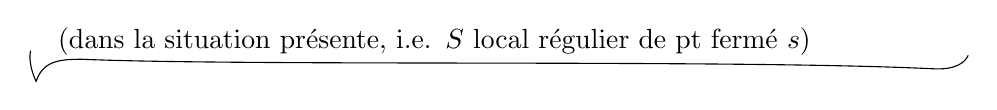
\begin{tikzpicture}
\node[anchor=south west,inner sep=0pt,outer sep=0pt,text width=0.94\linewidth,align=left] (addition) at (0,0) {\inserted{(dans la situation présente, i.e. $S$ local régulier de pt fermé $s$)}};
\handwritten{\draw[line width=0.4pt]
 ([xshift=-3.5mm,yshift=0.6mm]addition.south west)
 .. controls ([xshift=-3.8mm,yshift=-0.8mm]addition.south west)
 and ([xshift=-3.2mm,yshift=-2.5mm]addition.south west)
 .. ([xshift=-2.8mm,yshift=-3.3mm]addition.south west)
 .. controls ([xshift=-1.9mm,yshift=-0.6mm]addition.south west)
 and ([xshift=0.4mm,yshift=-0.5mm]addition.south west)
 .. ([xshift=3.0mm,yshift=-0.5mm]addition.south west)
 .. controls ([xshift=25mm,yshift=-1.4mm]addition.south west)
 and ([xshift=-28mm,yshift=-0.5mm]addition.south east)
 .. ([xshift=-3mm,yshift=-1.7mm]addition.south east)
 .. controls ([xshift=0mm,yshift=-1.9mm]addition.south east)
 and ([xshift=1.2mm,yshift=-0.9mm]addition.south east)
 .. ([xshift=1.6mm,yshift=0mm]addition.south east);}
\end{tikzpicture}%
}
\noindent une caractérisation d'un homomorphisme (7.17.4.1) ? \handwritten{(${}^1$)}

p.27, li.1 et 2 du bas : ``au-dessus'' et non ``au dessus''. Dire ``dans le normalisé'' au lieu de ``du normalisé''.

p.28 : dans la bibliographie, manque la référence Abhyankar sur la résolution des singularités des surfaces arithmétiques.

\handwritten{(${}^1$) Est-ce que 7.2 ne \unsure{x|se} généralise pas ?}

% Detached dark marks in the lower-right blank area; authored status and function uncertain.
\par\vspace*{0.27\textheight}
\noindent\hfill\parbox[c]{3mm}{\figure{\unsure{%
\begin{tikzpicture}[x=1mm,y=1mm]
\fill (-0.39,-0.02) .. controls (-0.44,0.18) and (-0.23,0.27) .. (-0.17,0.45)
 .. controls (0.01,0.59) and (0.15,0.29) .. (0.23,0.19)
 .. controls (0.48,0.13) and (0.43,-0.09) .. (0.19,-0.18)
 .. controls (0.05,-0.40) and (-0.17,-0.29) .. (-0.39,-0.02) -- cycle;
\fill (0.58,1.30) .. controls (0.66,1.49) and (0.84,1.48) .. (0.89,1.73)
 .. controls (0.97,1.93) and (1.13,1.72) .. (1.14,1.58)
 .. controls (1.32,1.44) and (1.25,1.24) .. (1.10,1.16)
 .. controls (1.01,0.97) and (0.75,1.08) .. (0.58,1.30) -- cycle;
\fill (-0.60,1.38) ellipse[x radius=0.15,y radius=0.16];
\end{tikzpicture}%
}}}\hspace*{0.04\linewidth}\par

% archive sheet number: 71
\clearpage
\scanpage{74}

\begin{flushright}
Massy le 3.11.1970\\
\end{flushright}

\noindent Cher Ferrand,\\

J'aimerais savoir si je peux compter sur ton exposé SGA 6 XI dans un avenir assez rapproché (diso\unsure{n|u|m|r} d'ici fin décembre). Dans le cas contraire, je pense qu'il serait préfé\deleted{é}r\deleted{\unsure{r}}able que je publie SGA 6 sans l'exposé XI. Il serait quand même raisonnable, après le travail que tu t'es tapé, que tu en fasses au moins un article d'exposition, et j'aimerais savoir alors où tu penses le publier, pour que je puisse y référer dans l'introduction à SGA 6.

Bien cordialement\\

% Isolated curved mark in the lower-right blank area, far below the closing.
% Its visible shape is retained; pen mark versus incidental surface trace remains uncertain.
\par\vspace*{0.43\textheight}
\noindent\hfill\parbox[c]{9mm}{\figure{\unsure{\handwritten{%
\begin{tikzpicture}[x=1mm,y=1mm]
\draw[line width=0.25pt] (0,5.35)
 .. controls (2.3,4.50) and (5.65,3.65) .. (7.20,2.20)
 .. controls (8.05,1.43) and (8.45,0.50) .. (8.00,0.15)
 .. controls (7.88,0.03) and (7.60,-0.06) .. (7.42,0.00);
\end{tikzpicture}%
}}}}\hspace*{0.025\linewidth}\par
% archive sheet number: 73
\clearpage
\scanpage{75}
% slanted
\reversemarginpar\margin{\shortstack[l]{\unsure{Joindre|joindre}\\SGA 7 \(\overline{\underline{\mathrm{VI}}}\) ?\\App. \(\overline{\underline{\mathrm{II}}}\)}}\normalmarginpar
\noindent\hfill Bures sur Yvette, le 21 octobre 1968\\

\noindent Cher Grothendieck,\\

En fait, il n'est pas nécessaire de faire de savants recollages de complexes cotangents pour prouver que

\noindent \uline{proposition} : \uline{Soit} \(X\) \uline{un espace analytique complexe compact}. \uline{Pour que} \(X\) \uline{soit un schéma}, \uline{il faut et suffit que} \(X_{\mathrm{red}}\) \uline{le soit}

On se ramène à \deleted{supposer} montrer que si \(X_0\) est défini par un Idéal de carré nul, soit \(\mathscr{N}\), de \(X\), alors
\[
 (X_0\text{ est un schéma})\ \Longrightarrow\ (X\text{ est un schéma})
\]

Soit \(E^{\mathrm{an}}(X_0,\mathscr{N})\) et \(E^{\mathrm{alg}}(X_0,\mathscr{N})\) les groupes analytiques et algébriques d'extensions infinitésimales de \(X_0\) par \(\mathscr{N}\). Soit enfin \(\unsure{K|\mathbb{K}}\) le complexe cotangent de \(X_0\), \uline{donné localement, dans la catégorie dérivée}. il s'obtient en plongeant \uline{localement} (Zariski, ou étale) \(X_0\) dans un \unsure{schéma} lisse \ldots\ et permet de définir
\begingroup
\makeatletter\tagsleft@true\makeatother
\[
 \mathscr{H}om(K,\mathscr{N})\qquad\text{et}\qquad
 \mathscr{E}xt^{1}\makebox[0pt][l]{\hspace{-0.20em}\raisebox{-1.8ex}[0pt][0pt]{\parbox[c]{1.5mm}{\figure{\unsure{%
 \begin{tikzpicture}[x=1mm,y=1mm,baseline=0pt]
 \fill[gray!75] (-0.28,-0.02) .. controls (-0.28,0.12) and (-0.11,0.27) .. (0.05,0.25)
 .. controls (0.19,0.23) and (0.29,0.06) .. (0.22,-0.03) -- cycle;
 \fill[gray!30] (0.62,0.08) ellipse[x radius=0.08,y radius=0.17,rotate=32];
 \end{tikzpicture}%
 }}}}}(K,\mathscr{N})\ .\tag*{(1)}
\]
\endgroup

Soit le diagramme :

\margin{\vspace*{1.4em}\figure{\unsure{%
\begin{tikzpicture}[x=1mm,y=1mm]
\fill (-0.22,-0.07)
 .. controls (-0.27,0.06) and (-0.16,0.16) .. (-0.08,0.17)
 .. controls (-0.04,0.30) and (0.06,0.25) .. (0.11,0.14)
 .. controls (0.25,0.10) and (0.27,-0.03) .. (0.15,-0.11)
 .. controls (0.04,-0.15) and (-0.15,-0.16) .. (-0.22,-0.07) -- cycle;
\fill (0.37,0.72)
 .. controls (0.34,0.85) and (0.44,0.95) .. (0.50,0.98)
 .. controls (0.54,1.10) and (0.65,1.11) .. (0.71,1.00)
 .. controls (0.83,0.94) and (0.77,0.85) .. (0.68,0.81)
 .. controls (0.73,0.69) and (0.64,0.62) .. (0.53,0.65)
 .. controls (0.44,0.63) and (0.38,0.65) .. (0.37,0.72) -- cycle;
\fill[gray!65] (0.20,-0.19) .. controls (0.22,-0.13) and (0.31,-0.23) .. (0.34,-0.34)
 .. controls (0.30,-0.46) and (0.18,-0.36) .. (0.20,-0.19) -- cycle;
\fill[gray!50] (0.47,-0.50) ellipse[x radius=0.06,y radius=0.08];
\end{tikzpicture}%
}}}

\diagram{\footnotesize
\begin{tikzcd}[ampersand replacement=\&,column sep=0.85em,row sep=1.6em]
 (2) \& 0 \arrow[r] \&
 H^{1^{\mathrm{alg}}}(X_0,\mathscr{H}om(K,\mathscr{N})) \arrow[r] \arrow[d] \&
 E^{\mathrm{alg}}(X_0,\mathscr{N}) \arrow[r,"\alpha"] \arrow[d] \&
 H^{0}(X_0,\mathscr{E}xt^{1}(K,\mathscr{N})) \arrow[d] \\
 \& 0 \arrow[r] \&
 H^{1^{\mathrm{an}}}(X_0,\mathscr{H}om(K,\mathscr{N})) \arrow[r] \&
 E^{\mathrm{an}}(X_0,\mathscr{N}) \arrow[r,"\beta"] \&
 H^{0^{\mathrm{an}}}(X_0,\mathscr{E}xt^{1}(K,\mathscr{N}))
\end{tikzcd}}


Vu les significations (locales) de (1), les lignes sont exactes ; par GAGA, les flèches verticales extrêmes sont des isomorphismes. Reste à \deleted{comparer les images de \mbox{\(\alpha\)} et \mbox{\(\beta\)}} montrer que \(\operatorname{Im}(\beta)\subset\operatorname{Im}(\alpha)\).
% archive sheet number: 74
\clearpage
\scanpage{76}
\noindent Soit donc \(U_i\) un recouvrement affine de \(X_0\), et
\[
 e\in H^{0^{(\mathrm{alg})}}(X_0,\mathscr{E}xt^1(K,\mathscr{N}))
\]
représenté par des classes d'isomorphies (algébriques) d'extensions \makebox[1.8em][c]{\raisebox{1.0ex}[0pt][0pt]{\parbox[b]{1.8em}{\figure{%

\begin{tikzpicture}[x=1mm,y=1mm,baseline=0pt]
\node[anchor=south,inner sep=0pt,outer sep=0pt] at (0,3.0) {$\inserted{U'_i}$};
\draw[line width=0.4pt] (-3.2,3.0)
 .. controls (-3.7,1.6) and (-2.4,1.2) .. (-1.2,1.0)
 .. controls (-0.5,0.8) and (-0.1,0.3) .. (0,0)
 .. controls (0.6,1.0) and (1.3,2.3) .. (2.3,2.6)
 .. controls (2.9,2.8) and (3.2,2.5) .. (3.7,2.6);
\end{tikzpicture}%
}}}} de \(U_i\) par \(\mathscr{N}\mid U_i\), classes d'isomorphies qui se recollent :

\[
 \text{soit }\unsure{\eta|n}_{ij}\text{ un isomorphisme}\qquad
 U'_j\mid U_i\cap U_j
 \xrightarrow{\sim}
 U'_{\unsure{i|j|k}}\mid U_i\cap U_j\ .
\]

L'obstruction à construire des \(\eta_{ij}\) \unsure{\deleted{d}t|t}els que \(\eta_{ij}\eta_{jk}=\eta_{ik}\) est donné par \(d_2\eta\) où \(d_2\) est une certaine flèche
\[
 d_2:H^0(X_0,\mathscr{E}xt^1(K,\mathscr{N}))\longrightarrow
 H^2(X_0,\mathscr{H}om(K,\mathscr{N}))
\]

La même construction marche dans le cas analytique, et on conclut par une nouvelle application de GAGA.

\uline{Rmq} 1 : itou pour les espaces algébriques, espaces rigides analytiques ; schémas formels

\deleted{\uline{\unsure{Rmq 2|Rmqs}}} :

\noindent\hfill Bien à toi\\
\null\hfill P. Deligne\\
% Signature written on a rising baseline.
\margin{\vspace*{2.5em}\figure{\unsure{%
\begin{tikzpicture}[x=1mm,y=1mm]
\fill (-0.17,-0.04)
 .. controls (-0.30,0.02) and (-0.29,0.16) .. (-0.16,0.21)
 .. controls (-0.12,0.39) and (0.04,0.41) .. (0.10,0.25)
 .. controls (0.26,0.24) and (0.32,0.08) .. (0.18,0.01)
 .. controls (0.16,-0.08) and (0.06,-0.08) .. (0.02,-0.20)
 .. controls (-0.04,-0.29) and (-0.14,-0.18) .. (-0.17,-0.04) -- cycle;
\fill (0.36,0.75)
 .. controls (0.21,0.80) and (0.26,1.01) .. (0.42,1.01)
 .. controls (0.49,1.18) and (0.61,1.11) .. (0.66,1.04)
 .. controls (0.77,1.01) and (0.81,0.87) .. (0.71,0.81)
 .. controls (0.69,0.68) and (0.49,0.64) .. (0.36,0.75) -- cycle;
\end{tikzpicture}%
}}}
% archive sheet number: 75
\clearpage
\scanpage{77}
% letterhead
\begin{center}
{\sffamily INSTITUT\\
DES HAUTES ÉTUDES SCIENTIFIQUES}\\[-0.4ex]
\rule{1.7cm}{0.5pt}
\end{center}

\figure{\footnotesize\begin{tikzpicture}
\node[anchor=west,inner sep=0pt,align=left] (haut) at (0,0) {
\(\overline{\underline{\unsure{\mathrm{VI}|\mathrm{VII}}}}\,
 1.11\ \text{\unsure{:|à}}\ 1.14\
 \text{\unsure{apres|après}}\ 1.15\,-\,1.22\ \text{? Refaire }1.14\ \text{?}\)\\[1.3ex]
\(\overline{\underline{\mathrm{VI}}}\)\quad appendice : la lettre Deligne 2 pages};
\draw[semithick] ([xshift=-.15em,yshift=.18ex]haut.north west)
 .. controls +(-.29em,-.26ex) and +(.12em,.50ex) .. ([xshift=-.28em,yshift=.79ex]haut.west)
 .. controls +(.12em,-.62ex) and +(.26em,.22ex) .. ([xshift=-.64em]haut.west)
 .. controls +(.49em,-.17ex) and +(.05em,.44ex) .. ([xshift=-.26em,yshift=-.82ex]haut.west)
 .. controls +(.02em,-.46ex) and +(-.23em,-.13ex) .. ([xshift=-.1em,yshift=-.1ex]haut.south west);
% A second lower contour is visible in the retraced brace.
\draw[thin] ([xshift=-.08em,yshift=.16ex]haut.west)
 .. controls +(-.18em,-.30ex) and +(-.15em,.50ex) .. ([xshift=-.04em,yshift=-.13ex]haut.south west)
 .. controls +(.05em,-.16ex) and +(.12em,-.05ex) .. ([xshift=.03em,yshift=-.02ex]haut.south west);
\node[inner sep=0pt] (sga) at ([xshift=-1.15cm,yshift=-.4ex]haut.west) {SGA 7};
\draw[thin] ([xshift=-.79cm,yshift=-.06cm]sga.center)
 .. controls +(.07cm,.45cm) and +(-.47cm,.03cm) .. ([xshift=.72cm,yshift=.64cm]sga.center)
 .. controls +(.04cm,-.47cm) and +(.38cm,.03cm) .. ([xshift=-.18cm,yshift=-.65cm]sga.center)
 .. controls +(-.40cm,0cm) and +(-.05cm,-.24cm) .. ([xshift=-.79cm,yshift=-.06cm]sga.center);
\end{tikzpicture}}

% slanted
\reversemarginpar\margin{\raisebox{-1.4\baselineskip}[0pt][0pt]{\shortstack[l]{faire un\\exposé\\\(\overline{\underline{\mathrm{XXIII}}}\) ?}}}\normalmarginpar
\figure{\footnotesize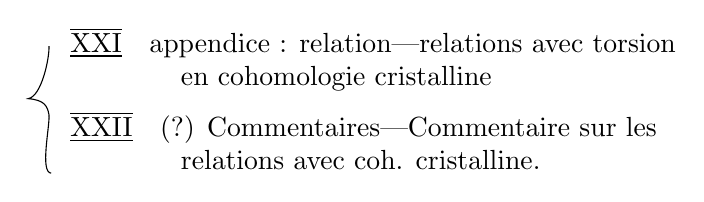
\begin{tikzpicture}
\node[anchor=west,inner sep=0pt,align=left] (bas) at (0,0) {
 \(\overline{\underline{\mathrm{XXI}}}\)\quad appendice : \unsure{relation|relations} avec torsion\\
 \hspace{4em}en cohomologie cristalline\\[1.5ex]
 \(\overline{\underline{\mathrm{XXII}}}\)\quad (?) \unsure{Commentaires|Commentaire} sur les\\
 \hspace{4em}relations avec coh. cristalline.};
\draw[thin] ([xshift=-.75em,yshift=-1.6ex]bas.north west)
 .. controls +(.02em,-1.0ex) and +(.48em,.18ex) .. ([xshift=-1.5em]bas.west)
 .. controls +(.6em,-.12ex) and +(-.06em,.72ex) .. ([xshift=-.75em,yshift=-1.35ex]bas.west)
 .. controls +(.04em,-.9ex) and +(-.42em,.05ex) .. ([xshift=-.67em,yshift=-.25ex]bas.south west);
\end{tikzpicture}}
% archive sheet number: 76
\clearpage
\scanpage{85}
\mspage{- 538 -}

\begin{center}
TABLE DES MATIERES
\end{center}

\noindent AVANT-PROPOS \dotfill

\noindent INTRODUCTION\dotfill

\noindent CHAPITRE \unsure{O|0} .- Préliminaires\dotfill

\noindent\quad \S\ 1. Foncteurs représentables\dotfill

\noindent\qquad 1.1. Foncteurs représentables\dotfill

\noindent\qquad 1.2. Produits fibrés dans une catégorie\dotfill

\noindent\qquad 1.3. Changement de base\dotfill

\noindent\qquad 1.4. Noyaux ; morphisme diagonal\dotfill

\noindent\qquad 1.5. Foncteurs adjoints\dotfill

\noindent\qquad 1.6. Structures algébriques dans les catégories\dotfill

\noindent\qquad 1.7. Morphismes fonctoriels représentables\dotfill

\noindent\quad \S\ 2. Compléments de topologie\dotfill

\noindent\qquad 2.1. Espaces irréductibles\dotfill

\noindent\qquad 2.2. Espaces localement noethériens\dotfill

\noindent\qquad 2.3. Ensembles quasi-constructibles et ensembles constructibles\dotfill

\begingroup
\reversemarginpar
\margin{\figure{\handwritten{\unsure{%
\begin{tikzpicture}[x=1mm,y=1mm]
\draw[line width=0.5pt]
 (0,6.80) .. controls (0.50,7.00) and (1.15,7.25) .. (1.62,7.15)
 .. controls (2.05,7.06) and (2.23,6.60) .. (2.13,6.12)
 .. controls (2.05,5.10) and (1.77,4.02) .. (1.46,2.77)
 .. controls (1.32,2.40) and (1.37,2.15) .. (1.69,2.10)
 .. controls (2.02,2.02) and (2.30,2.36) .. (2.55,2.18);
\draw[line width=0.5pt] (3.34,0.15) .. controls (3.64,0.28) and (3.91,0.22) .. (4.10,0.16);
\end{tikzpicture}%
}}}}
\endgroup
\figure{%
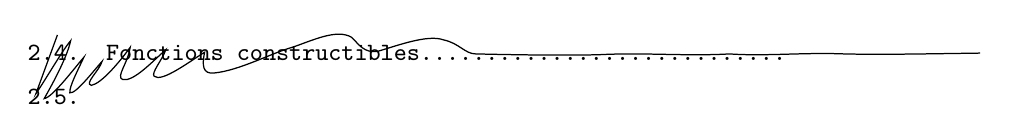
\begin{tikzpicture}[x=0.105mm,y=-0.105mm]
\node[anchor=base west,inner sep=0pt,outer sep=0pt,font=\ttfamily\small] at (13,41)
 {\deleted{2.4. Fonctions constructibles}\deleted{\mbox{............................}}};
\node[anchor=base west,inner sep=0pt,outer sep=0pt,font=\ttfamily\small] at (13,94)
 {\deleted{2.5.}};
% The deletion macros record state; this path records the observed freehand course.
\handwritten{\draw[line width=0.45pt]
 (49,10) -- (23,81)
 .. controls (31,70) and (56,27) .. (65,17)
 .. controls (60,40) and (38,78) .. (33,87)
 .. controls (43,86) and (72,47) .. (81,37)
 .. controls (74,52) and (63,73) .. (64,80)
 .. controls (71,82) and (93,53) .. (103,42)
 .. controls (100,53) and (81,69) .. (90,71)
 .. controls (102,69) and (124,43) .. (137,25)
 .. controls (135,43) and (119,61) .. (128,64)
 .. controls (141,67) and (164,42) .. (180,28)
 .. controls (176,40) and (162,56) .. (166,60)
 .. controls (175,68) and (209,42) .. (227,31)
 .. controls (224,46) and (224,58) .. (239,56)
 .. controls (269,53) and (308,32) .. (333,25)
 .. controls (357,17) and (387,2) .. (405,13)
 .. controls (414,22) and (420,32) .. (436,30)
 .. controls (460,23) and (497,9) .. (516,16)
 .. controls (535,20) and (542,33) .. (555,33)
 .. controls (601,34) and (652,35) .. (703,34)
 .. controls (758,31) and (808,36) .. (862,33)
 .. controls (906,36) and (951,31) .. (1001,33)
 .. controls (1046,34) and (1093,33) .. (1165,32);}
\end{tikzpicture}%
}

\noindent\qquad 2.4. Ensembles constructibles dans les espaces noethériens

\noindent\qquad 2.5? Fonctions constructibles\dotfill

\noindent\qquad 2.6. Parties très denses d'un espace topologique\dotfill

\noindent\qquad 2.7. Quasi-homéomorphismes\dotfill

\noindent\qquad 2.8. Espaces de Jacobson\dotfill

\noindent\qquad 2.9. Espace sobre associé à un espace topologique\dotfill

\noindent\qquad 2.10.Applications ouvertes en un point \dotfill

\noindent\quad \S\ 3. Compléments sur les faisceaux\dotfill

\noindent\qquad 3.1. Faisceaux à valeurs dans une catégorie\dotfill

\noindent\qquad 3.2. Préfaisceaux sur une base d'ouverts\dotfill

\noindent\qquad 3.3. Recollement de faisceaux\dotfill

\noindent\qquad 3.4. Images directes de préfaisceaux\dotfill

\noindent\qquad 3.5. Images réci\deleted{\unsure{r}}p\deleted{p}roque\unsure{s|\deleted{s}s|ss} de préfaisceaux\dotfill

\noindent\qquad 3.6. Faisceaux simples et faisceaux localement simples\dotfill

\noindent\qquad 3.7. Images réciproques de faisceaux de groupes ou d'anneaux\dotfill

% archive sheet number: 84
\clearpage
\scanpage{86}
\mspage{- 541 -}

\noindent\qquad 3.8. Morphismes universellement ouverts , universellement fermés , universellement bicontinus\dotfill

\noindent\qquad 3.9. Morphismes générisants\dotfill

\noindent\qquad 3.10. Morphismes submersifs et universellement submersifs

\noindent\quad \S\ 4. Sous-schémas et morphismes d'immersion .\makebox[0pt][l]{\hspace{0.35em}\raisebox{-0.5ex}[0pt][0pt]{\parbox[c]{1mm}{\figure{\unsure{%
\begin{tikzpicture}[x=1mm,y=1mm,baseline=0pt]
\fill (0,0) ellipse[x radius=0.13,y radius=0.22,rotate=-30];
\end{tikzpicture}%
}}}}} Schémas réduits\dotfill

\noindent\qquad 4.1. Sous-schémas\dotfill

\noindent\qquad 4.2. Morphismes d'immersion\dotfill

\noindent\qquad 4.3. Image réciproque d'un sous-schéma\dotfill

\noindent\qquad 4.4. Immersions locales et isomorphismes locaux\dotfill

\noindent\qquad 4.5. Schémas réduits\dotfill

\noindent\qquad 4.6. Existence d'un sous-schéma d'espace sous-jacent donné\dotfill

\noindent\quad \S\ 5. Morphismes séparés . Critères valuatifs\dotfill

\noindent\qquad 5.1. Diagonale d'un $S$-schéma\dotfill

\noindent\qquad 5.2. Morphismes et schémas séparés\dotfill

\noindent\qquad 5.3. Critères \deleted{\unsure{a|e}}de séparation\dotfill

\noindent\qquad 5.4. Morphismes schématiquement dominants et sous-schémas schématiquement denses\dotfill

\noindent\qquad 5.5. Critères valuati\deleted{\unsure{s|b}}fs\dotfill

\noindent\quad \S\ 6. Conditions de finitude relatives\dotfill

\noindent\qquad 6.1. Morphismes quasi-compacts et morphismes quasi-séparés\dotfill

\noindent\qquad 6.2. Morphismes localement de type fini et morphismes localement de présentation finie\dotfill

% Two unassigned points lie above the right-hand part of the 6.3 leaders.
\noindent\qquad 6.3. Morphismes de type fini et morphismes de présentation finie\dotfill\makebox[0pt][l]{\hspace{-0.08\linewidth}\raisebox{1.5ex}[0pt][0pt]{\parbox[c]{2mm}{\figure{\unsure{%
\begin{tikzpicture}[x=1mm,y=1mm,baseline=0pt]
\fill (-0.15,-0.05) .. controls (-0.18,0.12) and (-0.05,0.20) .. (0.05,0.14)
 .. controls (0.11,0.10) and (0.16,-0.04) .. (0.10,-0.09) -- cycle;
\fill (0.48,0.68) ellipse[x radius=0.13,y radius=0.20,rotate=-30];
\end{tikzpicture}%
}}}}}

\noindent\qquad 6.4. Schémas de \deleted{d}Jacobson et anneaux de \deleted{j}Jacobson\dotfill

\noindent\qquad 6.5. Schémas algébriques et localement algébriques\dotfill

\noindent\qquad 6.6. Détermi\deleted{j}nation locale d'un morphisme\dotfill

\noindent\qquad 6.7. Image directe d'un faisceau quasi-cohérent\dotfill

\noindent\qquad 6.8. Prolongement de sections de faisceaux quasi-cohérents

\noindent\qquad 6.9. Prolongement des faisceaux quasi-cohérents\dotfill

% The low contour is part of this uncertain correction cluster; it may be the old j foot.
\noindent\qquad 6.10.Image schémat\deleted{\unsure{l|t|j}}i\makebox[0pt][l]{\hspace{-0.25em}\raisebox{-1.0ex}[0pt][0pt]{\parbox[c]{1.4mm}{\figure{\unsure{%
\begin{tikzpicture}[x=1mm,y=1mm,baseline=0pt]
\fill (0,0) ellipse[x radius=0.09,y radius=0.10];
\fill (0.25,0.01) .. controls (0.36,0.12) and (0.47,0.10) .. (0.53,0.03)
 .. controls (0.64,0.13) and (0.75,0.07) .. (0.73,-0.02)
 .. controls (0.58,-0.08) and (0.38,-0.13) .. (0.25,0.01) -- cycle;
\end{tikzpicture}%
}}}}}que d'un schéma\unsure{,|.} Adhérence schématique d'un sous-schéma\dotfill

\noindent\qquad 6.11.Morphismes quasi-finis\dotfill

% archive sheet number: 85
\clearpage
